%% This is an example first chapter.  You should put chapter/appendix that you
%% write into a separate file, and add a line \include{yourfilename} to
%% main.tex, where `yourfilename.tex' is the name of the chapter/appendix file.
%% You can process specific files by typing their names in at the 
%% \files=
%% prompt when you run the file main.tex through LaTeX.
\chapter{Design}

In this chapter we argue all design decisions taken regarding the building of Redch. These are grounded on the detailed research explained in \ref{technology_research}. It extends the high-level architecture already outlined in \ref{fig:use_cases} further by first explaining the technology used: the programming languages, frameworks and most relevant libraries. Then, it presents the whole architecture of the system by describing each one of the components the system is comprised of.

The design explained below aims to be a solid ground and a first prototype for the Redch project. Therefore, not all ideas discussed in previous chapters may be included in the result of this master thesis. As a first step towards the final product it will serve to get insight...

Ruby has been chosen as the main language for the development of the project. This dynamic language focused on simplicity and productivity, is often regarded as developer performant. Due to its flexibility and similarity with natural language, along with the massive amount of libraries and frameworks available, it allows developers to write applications very quickly. However, this features hamper its execution performance.

\subsection{Physical Architecture}

The core idea of this architecture is to decouple the data producers from the data consumers by means of an asynchronous message queue enabling push capabilities in the consumption tier. It is compound of four different servers, as figure \ref{fig:physical_architecture} shows: An application server that receives the observations from the sensors and stores them in the database. That server is also responsible for publishing the observation into the messaging queue. Then, the messaging queue pushes them to the data consumption tier, where the app server sends them to the web clients.

\begin{figure}[H]
	\centering
	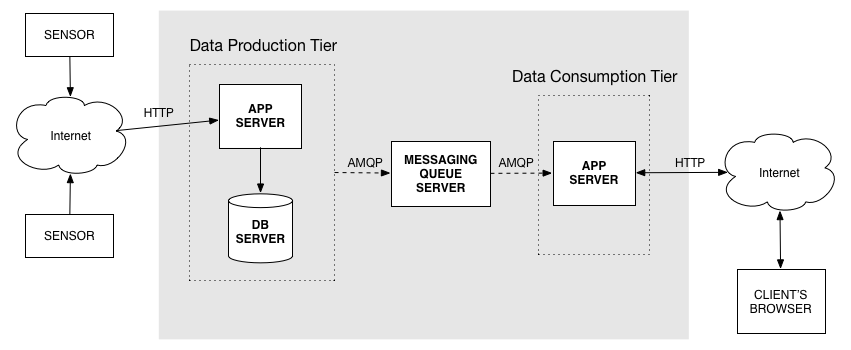
\includegraphics[width=\textwidth]{physical_architecture}
	\caption{Physical Architecture}
	\label{fig:physical_architecture}
\end{figure}

Such architecture brings a number of benefits, as outlined in \ref{technology_research}. First and foremost, each tier can easily scale out independently. In both tiers, high availability and increased throughput can be provided through redundancy \cite{Antwerp}, that is, adding more app servers. As for the database and the messaging queue, clusterizing them can provide better performance, increased throughput and storage capacity.

The loosely coupled architecture the messaging queue entails along with the benefits stated in \ref{message_passing} not only allows scaling horizontally, but also allows components to evolve independently. The only constraint is that both tiers must understand the Advanced Message Queuing Protocol (AMQP). On the other hand, given the wide adoption of such protocol, the particular messaging queue may be replaced without affecting any of the tiers.

Finally, a high-performance asynchronous messaging queue provides real-time capabilities to the system.

\subsection{Logical Architecture}

\subsubsection{Sensor}

As already stated in \ref{actors}, although we opt for a solution that may involve RaspberryPi, the development of the sensor device falls out of the scope of the project. Nonetheless, the system requires some sort of client in order to simulate its functioning in normal conditions.

\begin{figure}[H]
\begin{minipage}{.5\textwidth}
	\centering
	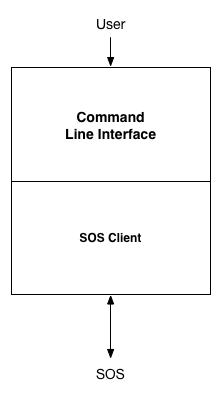
\includegraphics[width=.7\textwidth]{sensor_logic_view}
	\caption{Simulator's Logic View}
	\label{fig:sensor_logic_view}
\end{minipage}
\begin{minipage}{.5\textwidth}
	\centering
	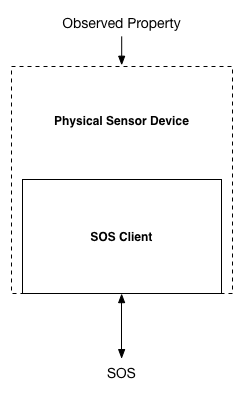
\includegraphics[width=.7\textwidth]{future_sensor_logic_view}
	\caption{Sensor's Logic View}
	\label{fig:future_sensor_logic_view}
\end{minipage}
\end{figure}

The CLI acts as a presentation layer that allows interaction with the underlying SOS API client hence, the particular features of the sensor can be simulated. Additionally, with this approach the SOS client can be reused as a logic component within the final sensor device.

\subsubsection{Messaging Queue}

The messaging queue is the central component which drives the data throughout the system. As a consequence, it determines the architecture of all other components. A detailed list of most known messaging queue systems has been given in \ref{message_passing}. All of them are high-performant, but usually message queues aren't the system's bottleneck, but message consumers slowed down by database queries or backend systems.

Then, the choice of an specific message queue depends on the amount of client libraries available, particularly for the languages used it in the project, its clustering support and the complexity of installation and management. It is also important that the chosen queue has enough high-quality online resources to help with the integration. RabbitMQ, with a rich management web UI and exhaustive documentation including a clustering guide, is the one that best fits our requirements.

This decision impacts on the design of the data producers and consumers, which must integrate with RabbitMQ using the AMQP protocol. This will be discussed further in following sections.


\subsubsection{Sensor Observation Service}

Given the CREAF's determination towards the SWE initiative and its involvement in Open-source GIS community it is important to make use of the Sensor Observation Service (SOS). To do so, we opt for 52ºNorth SOS 4.0, the leading open-source implementation already integrated by many research institutions throughout the world. In this regard, great efforts are underway to bring last web standards to the OGC implementations, which may be worth checking out in order to include them in Redch project. This is the case of 52ºNorth SOS 4.0. While this project uses its beta version, the final version has been released less than three months before this writing.

As fully discussed in \ref{interoperability}, SOS provides the level of interoperability the project requires.

The SOS specification structures the service with a core and four extensions: Transactional, Enhanced operations, Result handling and bindings. Together, all extensions provide CRUD functionality for sensors, observations and results.

With regard to the bindings only SOAP and KVP are defined in the specification. Additionally, 52ºNorth SOS 4.0 implements a RESTful binding as part of the bindings extension, which our SOS client will use. By choosing this binding, we aim to build a lightweight and stateless service client that can run in a resource-constrained sensor device.

In order to integrate with RabbitMQ, a component that handles the data delivery to the messaging queue must be developed and included in the SOS. Once the observation has been stored in the database, this component publishes a message with the observation into the queue. Its logical architecture is as figure \ref{fig:amqp_extension} shows.

\begin{figure}[p]
	\centering
	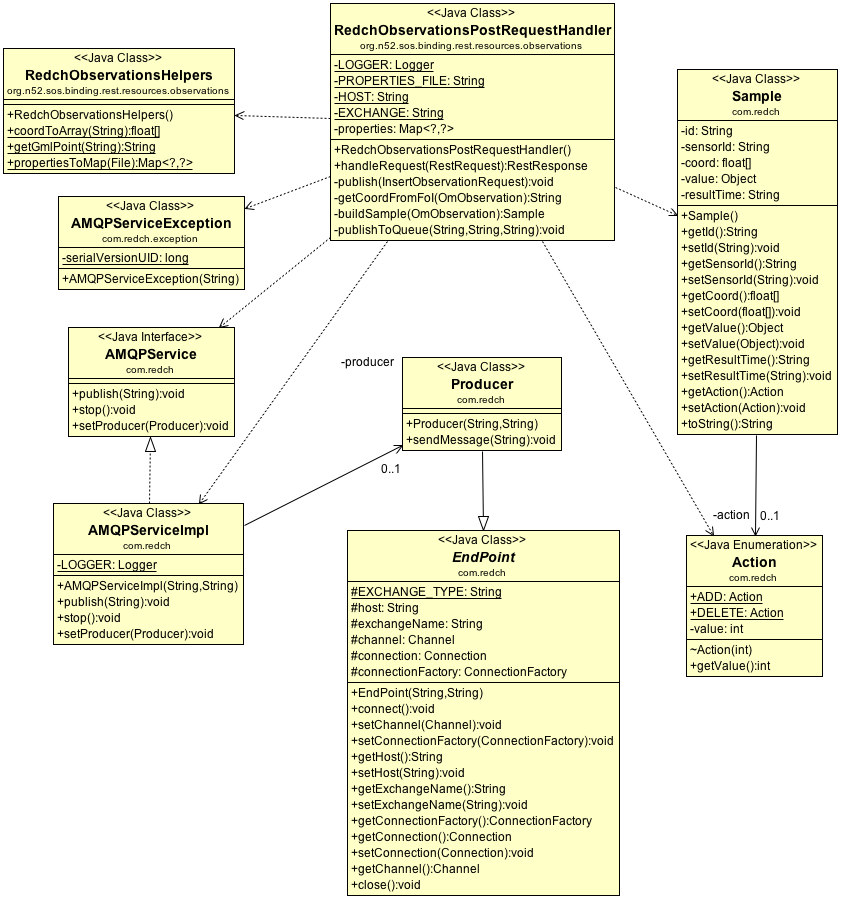
\includegraphics[width=\textwidth]{amqp_extension}
	\caption{SOS AMQP extension}
	\label{fig:amqp_extension}
\end{figure}

\subsubsection{Database}

52ºNorth's implementation uses Hibernate and Hibernate Spatial persistence framework to allow changing the underlying database management system and database model, which currently supports PostgreSQL/PostGIs, Oracle/Oracle spatial, MySQL and SQL Server DBMSs. Although we have chosen PostgreSQL, the GIS industry standard, Redch may benefit from the integration of some sort of NoSQL solution.

The system is characterised by an ever growing data set, with small data units. That is, the system is write-intensive and I/O-bound. Given this features, in a real-world scenario Redch may take advantage of NoSQL massive scalability and its higher performance and scalability. Furthermore, in this project the impact of relaxed consistency may not be as high as in other systems where high reliability is required.

The time constraints, however, do not allow to explore this possibility since it would require to migrate the relational schema to a non-relational one. In addition, this prototype will deal with a limited number of sensors for testing purposes only.


\subsubsection{Web Application}

impact on client of AMQP, SSE. Async app server. Reactor pattern.